% GNUPLOT: LaTeX picture with Postscript
\begingroup
  \makeatletter
  \providecommand\rotatebox[2]{#2}%
  \@ifundefined{ifGPcolor}{%
    \newif\ifGPcolor
    \GPcolortrue
  }{}%
  \@ifundefined{ifGPblacktext}{%
    \newif\ifGPblacktext
    \GPblacktexttrue
  }{}%
  % define a \g@addto@macro without @ in the name:
  \let\gplgaddtomacro\g@addto@macro
  % define empty templates for all commands taking text:
  \gdef\gplbacktext{}%
  \gdef\gplfronttext{}%
  \makeatother
  
  \setlength{\unitlength}{1cm}%
  \begin{picture}(23.8,16)%
    \gplgaddtomacro\gplbacktext{%
        \put(0,1.75){\makebox(0,0)[r]{\strut{} $u_6$}}%
        \put(0,4.25){\makebox(0,0)[r]{\strut{} $u_5$}}%
        \put(0,6.75){\makebox(0,0)[r]{\strut{} $u_4$}}%
        \put(0,9.25){\makebox(0,0)[r]{\strut{} $u_3$}}%
        \put(0,11.75){\makebox(0,0)[r]{\strut{} $u_2$}}%
        \put(0,14.25){\makebox(0,0)[r]{\strut{} $u_1$}}%
        \put(2.4,16){\makebox(0,0)[cr]{\strut{} $y_1$}}%
        \put(6.2,16){\makebox(0,0)[cr]{\strut{} $y_2$}}%
        \put(10,16){\makebox(0,0)[cr]{\strut{} $y_3$}}%
        \put(13.8,16){\makebox(0,0)[cr]{\strut{} $y_4$}}%
        \put(17.6,16){\makebox(0,0)[cr]{\strut{} $y_5$}}%
        \put(21.4,16){\makebox(0,0)[cr]{\strut{} $y_6$}}%
        \put(0.5,0.25){\line(1,0){22.8}}
        \put(0.5,0.15){\line(0,1){0.2}}
        \put(4.3,0.15){\line(0,1){0.2}}
        \put(8.1,0.15){\line(0,1){0.2}}
        \put(11.9,0.15){\line(0,1){0.2}}
        \put(15.7,0.15){\line(0,1){0.2}}
        \put(19.5,0.15){\line(0,1){0.2}}
        \put(23.3,0.15){\line(0,1){0.2}}
        \put(2.4,0){\makebox(0,0)[c]{\strut{}  \footnotesize $1 d$}}%
        \put(6.2,0){\makebox(0,0)[c]{\strut{} \footnotesize $1 d$}}%
        \put(10,0){\makebox(0,0)[c]{\strut{} \footnotesize $1 d$}}%
        \put(13.8,0){\makebox(0,0)[c]{\strut{} \footnotesize $5000 s$}}%
        \put(17.6,0){\makebox(0,0)[c]{\strut{} \footnotesize $5000 s$}}%
        \put(21.4,0){\makebox(0,0)[c]{\strut{} \footnotesize $5000 s$}}%
    }%
    \gplgaddtomacro\gplfronttext{%
    }%
    \gplbacktext
    \put(0.5,0.5){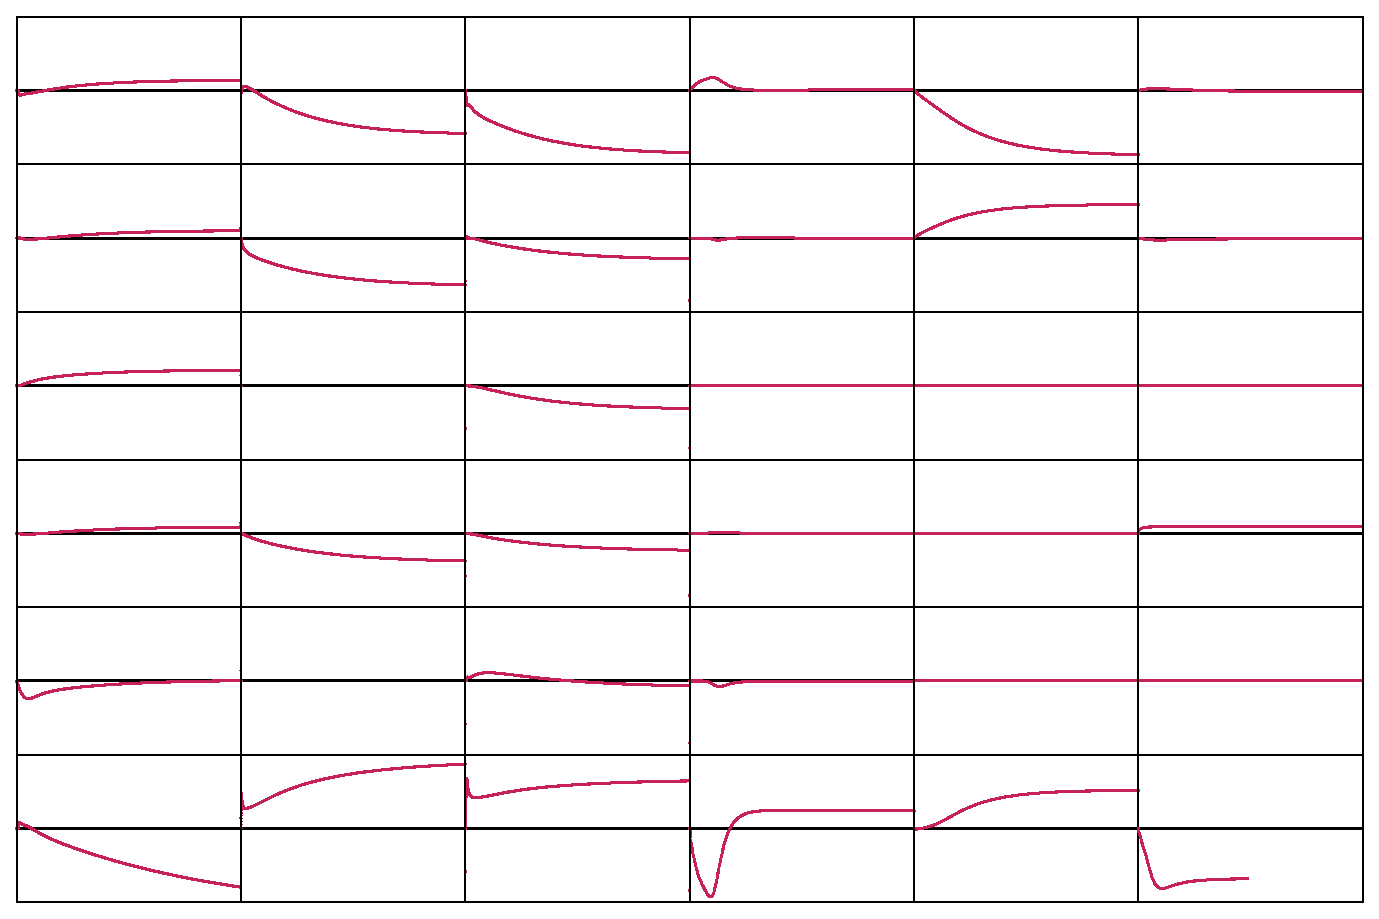
\includegraphics{GNUPlot/B1_Plot}}%
    \gplfronttext
  \end{picture}%
\endgroup
